\documentclass[journal=jpclcd,manuscript=article,articletitle=true,layout=twocolumn]{achemso}

\usepackage{amsmath}
\usepackage{amssymb}
\usepackage{latexsym}
\usepackage{graphicx}
\usepackage{epsfig,epsf,rotating}
\usepackage{indentfirst}
\usepackage{epstopdf}
\usepackage{xcolor}
\usepackage{multirow}
\usepackage{tabularx}
\usepackage{ctable}
\usepackage{textcomp}
\usepackage[version=4]{mhchem}
\usepackage{amsmath}

\usepackage{upgreek}
\newcolumntype{C}{>{\centering\arraybackslash}X}
\usepackage{nicefrac}

\addtolength{\tabcolsep}{-3pt}

\newcommand{\myemph}[1]{\textcolor{red}{\emph{#1}}}

\title{Polarizability Plays a Decisive Role in Modulating Association Between Molecular Cations and Anions\footnote{
Notice:  This manuscript has been authored by UT-Battelle, LLC, under contract DE-AC05-00OR22725 with the US Department of Energy (DOE). The US government retains and the publisher, by accepting the article for publication, acknowledges that the US government retains a nonexclusive, paid-up, irrevocable, worldwide license to publish or reproduce the published form of this manuscript, or allow others to do so, for US government purposes. DOE will provide public access to these results of federally sponsored research in accordance with the DOE Public Access Plan (http://energy.gov/downloads/doe-public-access-plan).}}

\author{Chase~E.~Herman}
\affiliation{Department of Chemical and Biomolecular Engineering, 150 Academy St., University of Delaware, Newark, DE 19716, USA}

\author{Arjun~Valiya~Parambathu}
\affiliation{Department of Chemical and Biomolecular Engineering, 150 Academy St., University of Delaware, Newark, DE 19716, USA}

\author{Dilip~N.~Asthagiri}
\affiliation{Oak Ridge National Laboratory, 1 Bethel Valley Rd., Oak Ridge, TN 37830, USA}
\email{asthagiridn@ornl.gov}

\author{Abraham~M.~Lenhoff} %  \corref{cor1}
\affiliation{Department of Chemical and Biomolecular Engineering, 150 Academy St., University of Delaware, Newark, DE 19716, USA}
\email{lenhoff@udel.edu}


\begin{document}
    \begin{abstract}

Electrostatic interactions involving proteins depend not just on the ionic charges involved but also on their chemical identities. Here we examine the origins of incompletely understood differences in the strength of association of different pairs of monovalent molecular ions that are relevant to protein-protein and protein-ligand interactions. Cationic analogues of the basic amino acid side chains are simulated along with oxyanionic analogues of cation-exchange (CEX) ligands and acidic amino acids. Experimentally observed association trends with respect to the cations, but not anions, are captured by a non-polarizable model. An effective continuum correction to account for electronic polarizability can capture both trends better, but at the expense of fidelity to the underlying free energy landscape for ion-pair association. A polarizable model proves decisive in capturing experimentally-suggested trends with respect to both cations and anions; critically, the free energy landscape for ion-pair association is itself altered, thus altering configurational sampling. 

\begin{tocentry} 
    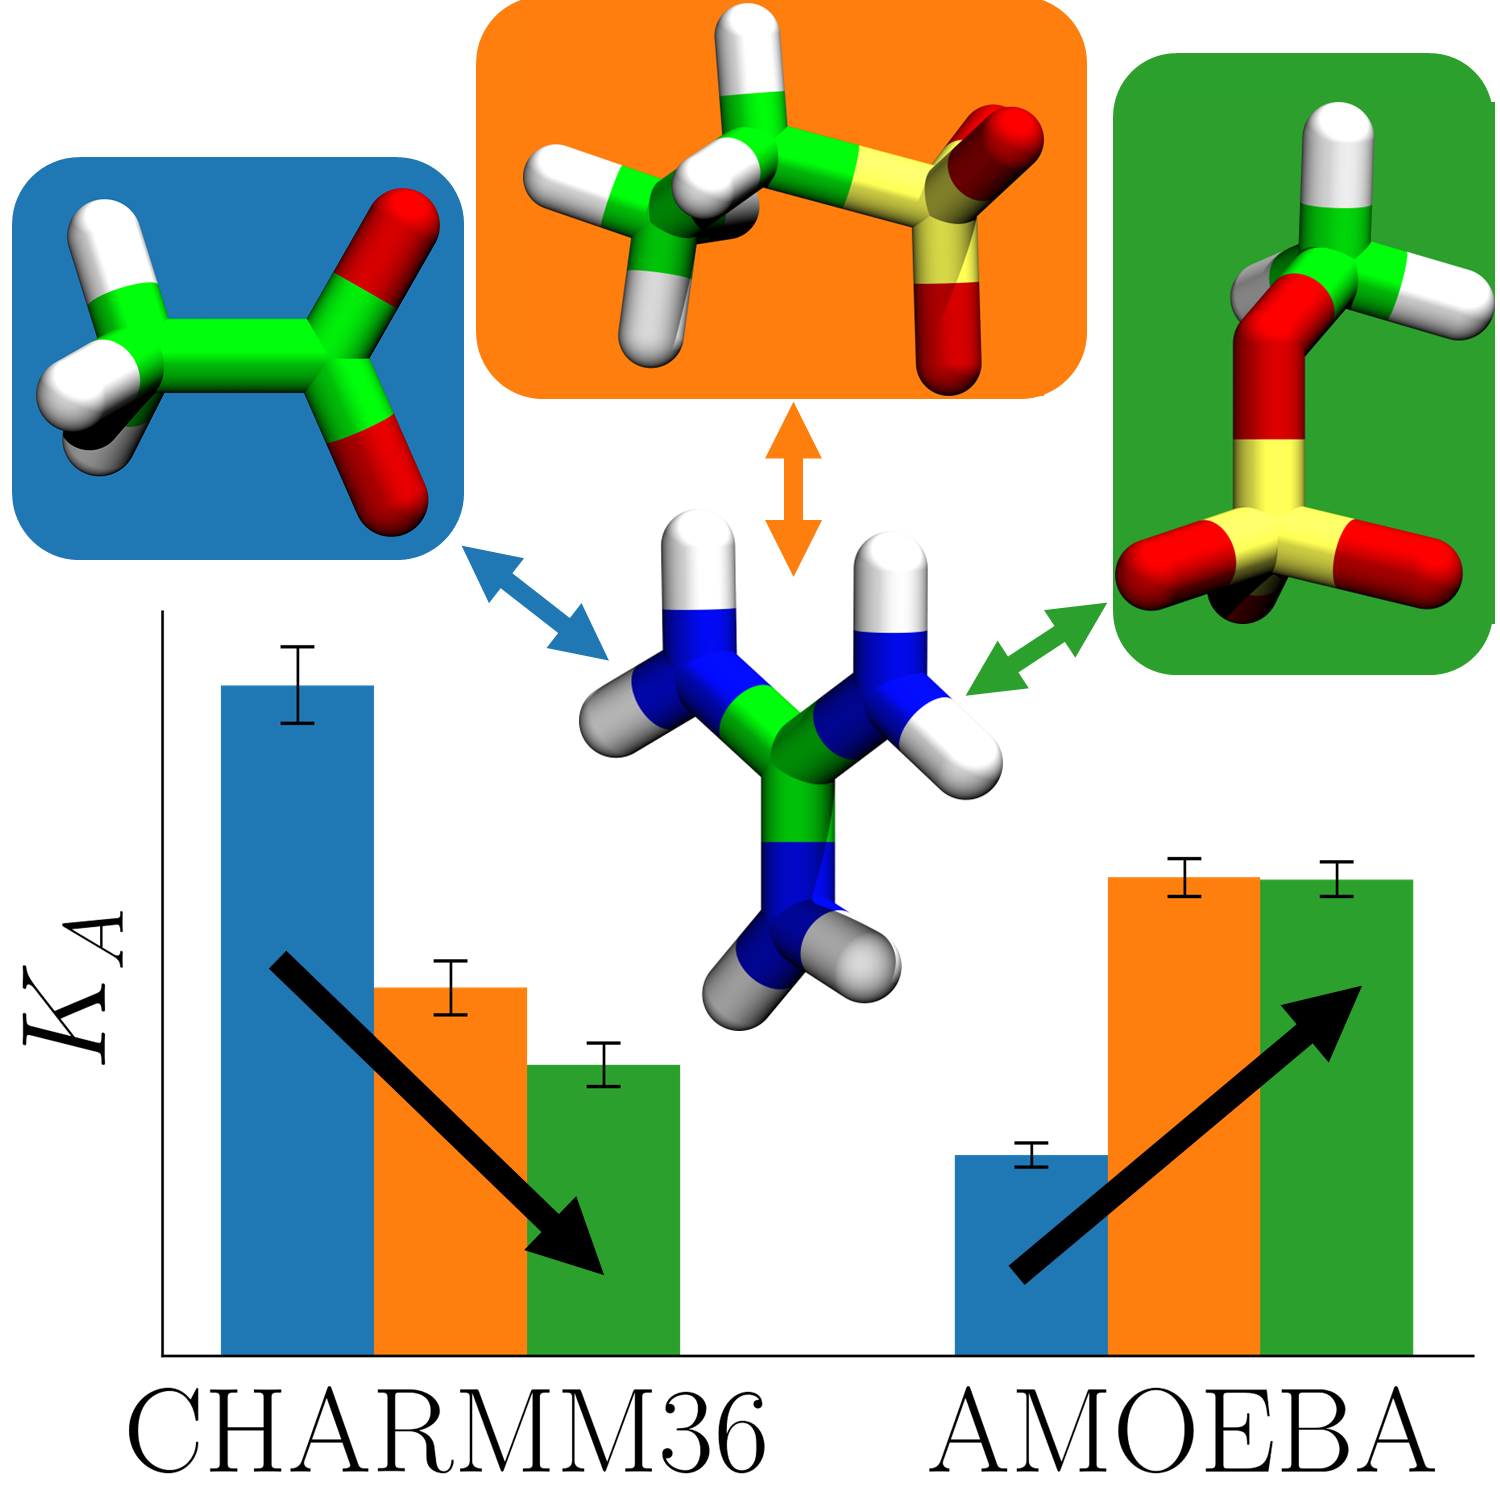
\includegraphics[height=5cm]{final_images/ToC.png} 
\end{tocentry}

\end{abstract}


\maketitle

Interactions among charged groups in aqueous solution are widely implicated in protein structural stabilization, biomolecular recognition and surface adsorption.\cite{Haggerty1991, Roberts2014, Luo1999} Among the specific phenomena of interest to this work is the longstanding puzzle that protein adsorption in cation-exchange (CEX) chromatography is known to be stronger on resins that are decorated with sulfate or sulfopropyl ligands than on resins with carboxymethyl ligands, despite the fact that the ligands bear the same formal charge and may be present on equivalent base matrices at comparable immobilization densities.\cite{DePhillips2001, Asthagiri2000} A related puzzle is the stronger binding to a heparin affinity resin of arginine than lysine 7-mers.\cite{Fromm1995} Uncovering the physics that underlie these observations on systems of broad scientific and technological interest still remains largely an open problem. 

Given the ionic nature of the constituents noted above, it is a natural first step to model the physics relying solely on electrostatics whilst ignoring the molecular nature of the solvent. Continuum solvent approaches have been enormously influential in guiding our thinking but they treat hydration phenomena only approximately and are unable to resolve puzzles such as those noted above\cite{Warshel2006, Ren2012, Koehl2006, Gray2018, Sun2016, Asthagiri2021b, Gunsteren2006}. It is necessary to account better for the underlying physics. 

\begin{figure}[ht]
    \begin{center}
        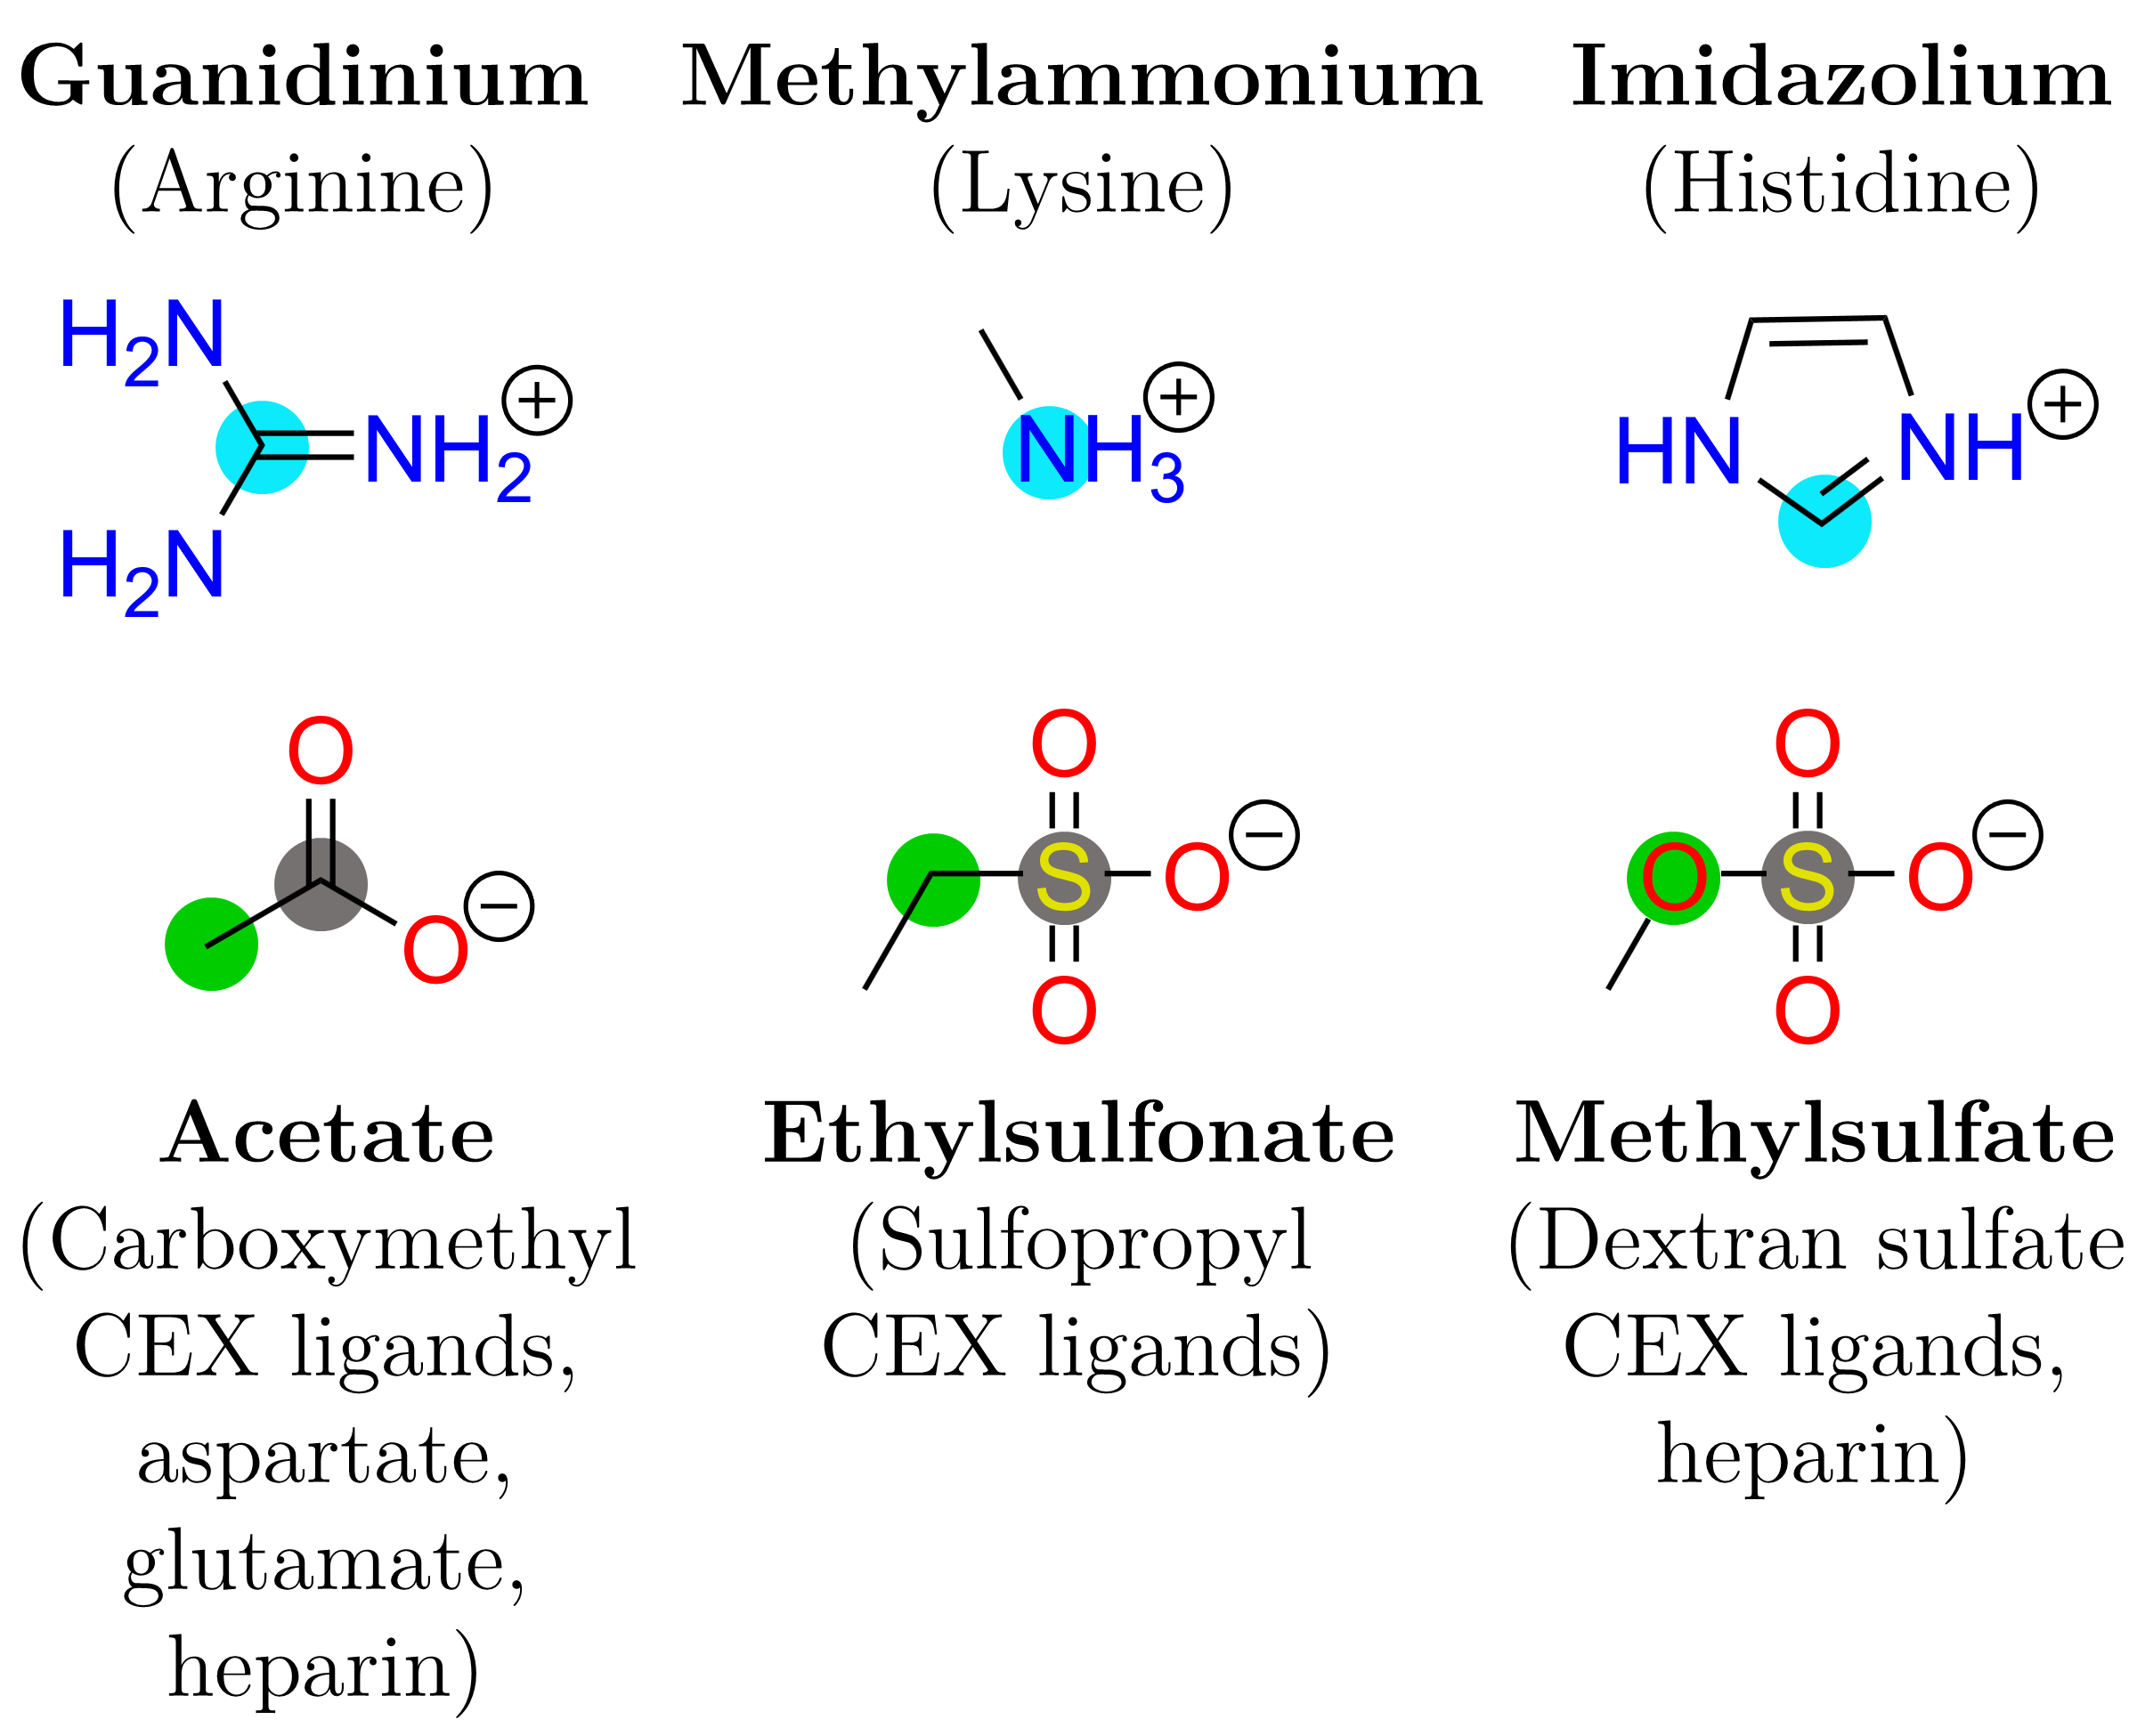
\includegraphics[width=\columnwidth]{final_images/Figure1.png}
        \caption{Cationic analogues (top) of the basic (i.e., positively charged) amino acid side chains and oxyanionic analogues (bottom) that were simulated in this work and are relevant to cation-exchange (CEX) chromatography, protein-protein interactions and protein-heparin interactions. Ion-pair separation distances $r$ were measured between the atoms that are highlighted in blue and grey circles and the coordinate $\theta$ was defined as the angle between the atoms that are highlighted in blue, grey and green circles.} 
        \label{fig:schematic}
    \end{center}
\end{figure}

All-atom molecular dynamics (MD) can in principle capture the balance between direct and indirect solvent-mediated intermolecular interactions.  However, classical non-polarizable force fields (FFs) are generally known to overestimate the strength of ion-pair interactions.\cite{Debiec2014, Debiec2016, Mason2019a} This may be attributable to the partial inclusion of polarization implicitly in the parameterization of water models but not in ion models.\cite{Dijon2020} To fix this disparity in the treatment of the solvent versus the ion, it has been suggested that ion charges be scaled by a constant factor of $1/\sqrt{\varepsilon_{el}} \sim 0.75$, where $\varepsilon_{el} \sim 1.78$ represents the high-frequency dielectric constant of water.\cite{Leontyev2011, Dijon2020}. Results using this so-called  electronic continuum correction (ECC) appear to better capture the strength of ion-pairing in solution. However, relative to the parent FF, the ECC complicates the estimation of solute hydration free energies \cite{Dijon2020} and may also err in describing intermolecular interactions at large separations.\cite{McDaniel2018} 
 
  \begin{figure*}[ht!]
    \begin{center}
        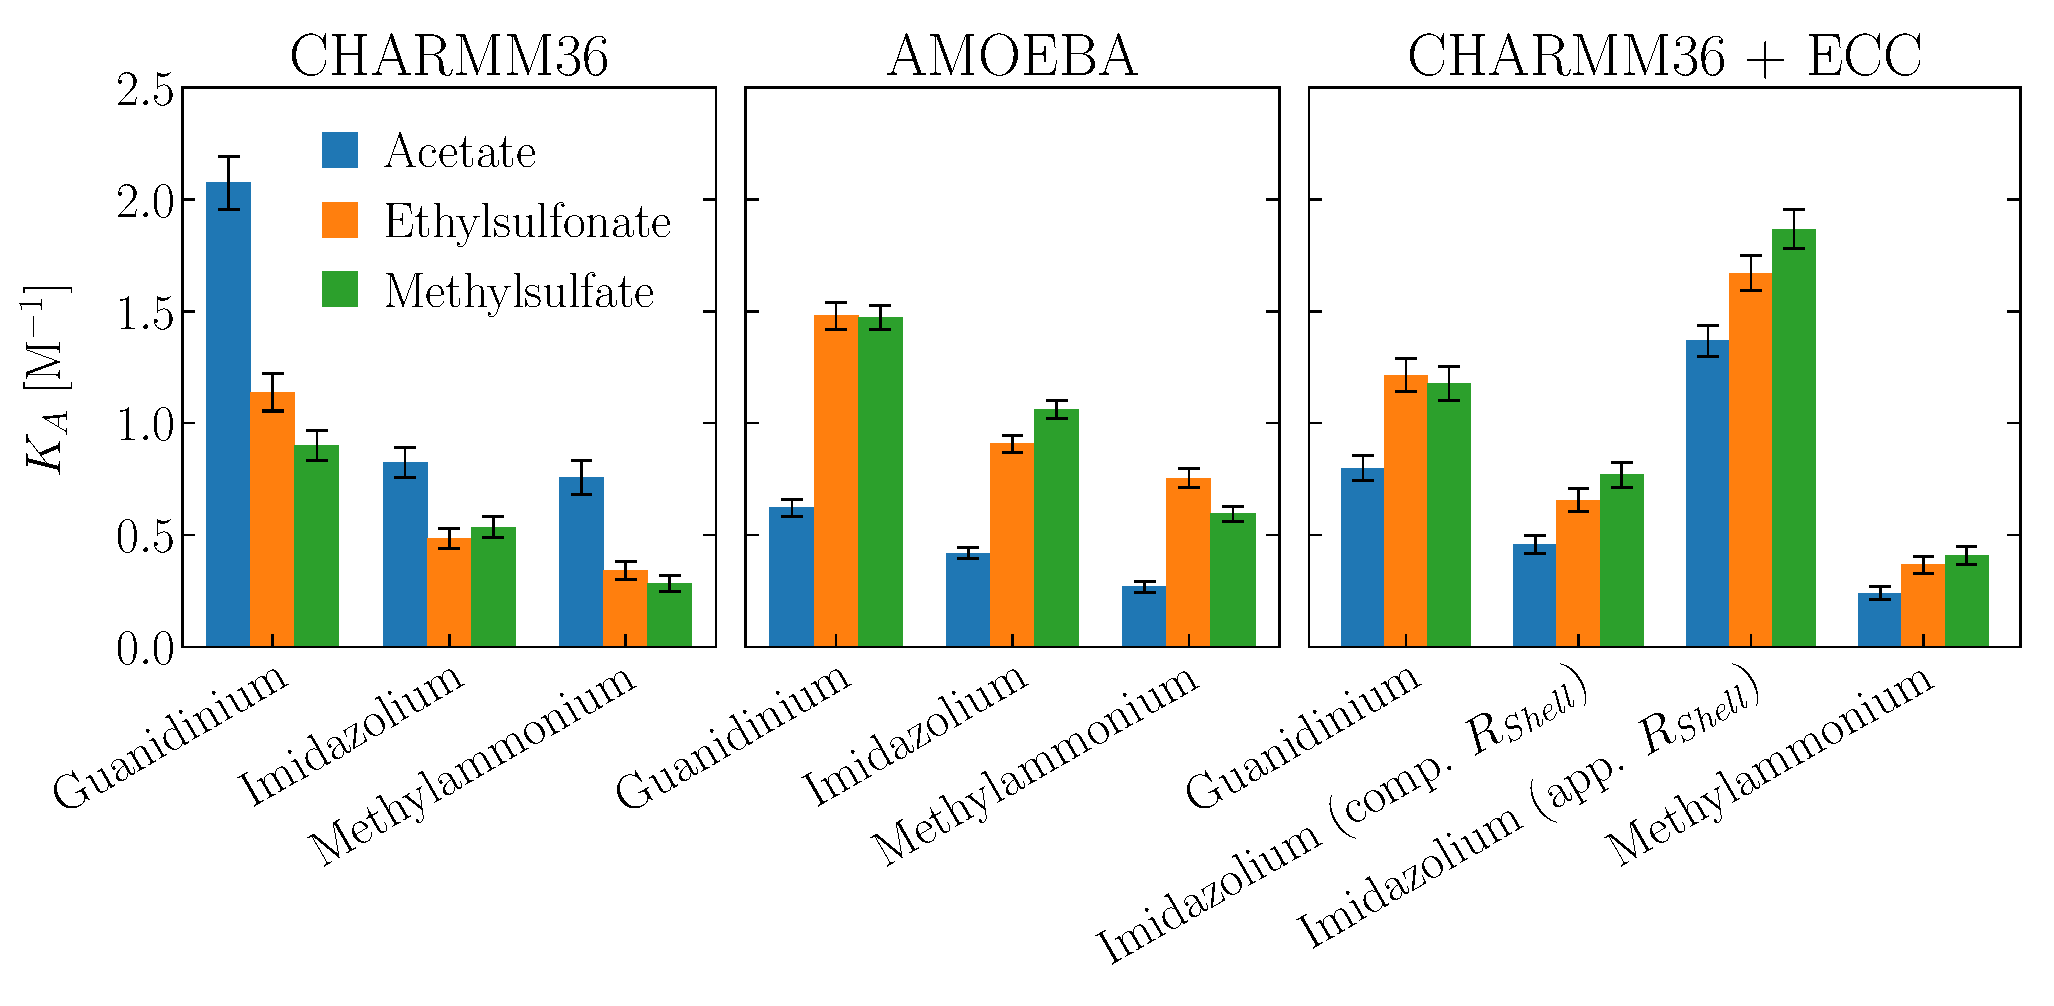
\includegraphics[width=\textwidth]{final_images/Figure2.eps}
        \caption{Association constants ($K_A$) obtained from the simulated interaction of cations (abscissa) with anions (bars) at a concentration of $\sim$ 0.5 M using different force fields (panels). Error bars represent $2\times$ the standard error of the mean and show that simulations are sufficiently converged to permit $K_A$ comparisons. ECC refers to the electronic continuum correction. For CHARMM36~+~ECC imidazolium systems, ``comp." and ``app." refer to comparable and apparent $R_{Shell}$ values that correspond to contact pair and solvent-separated PMF minima (Fig.~S1). Data are given in Table~S1.} 
        \label{fig:Ka_bar_plot}
    \end{center}
\end{figure*}	 

Here we assess the ability of a classical FF (CHARMM36\cite{Huang2013}) with and without the ECC as well as a polarizable model (AMOEBA\cite{Shi2013}) to explain the two puzzles noted above. Our previous work treated the solute at a quantum chemical level and the solvent as a continuum;\cite{Asthagiri2000} that effort captured some of the effects qualitatively, albeit with much uncertainty given the study's limited configurational exploration. Following that work, here we model analogues of oxyanionic CEX ligands (i.e., negatively charged acetate, methylsulfate and ethylsulfonate for carboxymethyl, dextran sulfate and sulfopropyl resins, respectively) interacting with comparable analogues of the basic amino acid side chains (i.e., positively charged guanidinium, methylammonium and imidazolium for arginine, lysine and histidine residues, respectively) (Fig.~\ref{fig:schematic}); acetate is of course also a model for the acidic (i.e., negatively charged) amino acid side chains. Focusing on ligands alone allows us to study physically critical interactions more thoroughly. The insights thus derived also have broad relevance to modeling protein interactions as well as ionic liquids.

\textbf{Association constants:} Unbiased simulations were performed for each anion-cation pair at a concentration of $\sim$ 0.5 M to compute potential of mean force (PMF) profiles (Supplementary Figure~S1); association constants $K_A$ were calculated as\cite{Zhu2012, Shi2017}
\begin{eqnarray}
K_{A} = \frac{1}{K_{D}} = 4 \pi \int_{0}^{R_{Shell}} r^2 e^{-w(r)/k_B T} \; dr
\label{eqn:Ka}
\end{eqnarray}
where $r$ and $w$ refer to the separation distance and the PMF, respectively, and the ions are considered to be associated for $r < R_{shell}$. The location of the first maximum in the PMF was chosen as $R_{shell}$,\cite{Shi2017} which separates the contact ion-pair from the solvent-separated ion pair and occurs at $r \sim 6$~{\AA} (Table~S1). The association constant may be alternatively obtained by counting associated and dissociated ion pairs in simulation trajectories,\cite{Debiec2014} but straightforward PMF integration is used here to avoid bookkeeping ambiguities related to multiply-associated ion pairs. 

Figure~\ref{fig:Ka_bar_plot} shows that both CHARMM36 and AMOEBA capture the expected $K_A$ rank order in cations (i.e., guanidinium $>$ imidazolium $>$ methylammonium) based on retention data of individual amino acids on sulfonate resins;\cite{Wang1989, Moore1958} the order is also consistent with the Lys and Arg oligomer retention in heparin affinity chromatography.\cite{Fromm1995} Although confounded by protein structural details, this order is furthermore consistent with the stronger retention of lysozyme (which is Arg-rich) than cytochrome \emph{c} (which is Lys-rich) on several CEX resins, which continuum electrostatics models may not be able to capture.\cite{DePhillips2001, Yao2005} CHARMM36 with the ECC generally captures the cation order, although the ECC tends to understructure the PMF profiles relative to AMOEBA (Fig.~S1). This is especially the case for imidazolium systems, making the definition of $R_{Shell}$ somewhat unclear. For this reason, comparable and apparent $R_{Shell}$ values are used in Figure~\ref{fig:Ka_bar_plot} that correspond approximately to contact and solvent-separated ion pairs. 

The more revealing comparisons are among the anions: CHARMM36 incorrectly predicts stronger cation interactions with acetate than with the sulfur-containing ligands. AMOEBA and the ECC both correct this trend to be consistent with the experimentally observed rank order of CEX resin retentivities. Two competing features stand out. From the perspective of the ions, relative to AMOEBA, CHARMM36 \emph{over}-stabilizes the interactions with acetate and \emph{under}-stabilizes the interactions with the sulfur-containing anions  (Fig.~S1). From the perspective of the solvent, relative to AMOEBA, CHARMM36 predicts \emph{weaker} acetate-water interactions but \emph{stronger} water interactions with the sulfur-containing anions (Fig.~S3). The ECC brings the classical model $K_A$ predictions closer to those of AMOEBA but sometimes at the expense of fidelity to the underlying PMF for ion-ion and ion-water association (Figs.~S1 and~S3). However, the ECC results could possibly be improved (i.e., made more like AMOEBA) by optimizing the charge scaling factor\cite{Dijon2020} or re-developing van der Waals parameters for the ion atoms that have scaled charges. Thus while general conclusions about the potential utility of charge scaling cannot be drawn from these data, it can be observed that implementing the ECC strategy effectively may be nontrivial. 

The rank-order comparisons of association constants that were presented above fulfill the objective of identifying what physics are required to treat biomolecular CEX interactions with at least qualitative fidelity. Several ambiguities obfuscate more rigorous quantitative comparisons between these results and experiment, a salient one of which is that the effective local concentration of negatively charged groups on CEX resin surfaces are generally unknown. However, guanidinium acetate association has been investigated in two independent potentiometric studies.\cite{Tanford1954, Haake1977} Association constants were inferred in those studies from an induced shift in the ionization constant of acetic acid when guanidinium was substituted for a third-party cation. However, the interpretation of the resulting data was predicated on the questionable assumption that the third-party cation does not complex with acetate. $K_A$ was independently estimated to be $\sim$~0.5~M$^{-1}$ and 0.37~M$^{-1}$,\cite{Tanford1954, Haake1977} but the ionic strength (IS) was uncontrolled in the first study,\cite{Tanford1954} which obfuscates the result because $K_A$ is expected to decrease with IS due to electrostatic screening. The IS was fixed at 1.02~M in the second study\cite{Haake1977} and the experimental value of 0.37~M$^{-1}$ is of comparable magnitude but appropriately lower than the AMOEBA prediction of 0.62~M$^{-1}$, which was obtained for guanidinium acetate at an IS of $\sim$~0.5~M. A comparable measurement of the interaction between butylammonium and acetate (0.31~M$^{-1}$ at 1.02~M IS)\cite{Haake1977} is also similar to the AMOEBA prediction for the methylammonium acetate system (0.27~M$^{-1}$ at $\sim$~0.5~M IS). All of these quantitative comparisons are intended simply to verify that the predicted $K_A$ values are of a reasonable magnitude; the rank-order comparisons are of greater importance to the chromatographic retentivity trends under investigation. The data from acetate simulations are also similar to previous computational results,\cite{Mason2019a, Debiec2014, Debiec2016} including a difference that was observed in classical simulations of guanidinium acetate using a different FF with and without the ECC (Fig.~S4).\cite{Mason2019a}

\textbf{Cross-FF analysis:} To assess whether the dissimilarities between the CHARMM36 and AMOEBA results were due to polarizability or simply a difference in the treatment of permanent electrostatics, a cross-FF analysis was performed in which the \emph{in vacuo} interaction energies between all ion pairs in AMOEBA simulation trajectories were analyzed retrospectively using both the CHARMM36 and AMOEBA FFs. This permitted an applied comparison of FF parameterization without any differences in configurational sampling. For each FF used in the analysis, the data were ensemble-averaged as a function of the separation distance $r$; Figures~S5-S7 show the decomposition of the \emph{in vacuo} interaction energy into permanent electrostatic ($U_{Elect}$), van der Waals ($U_{VdW}$) and polarization ($U_{Polar}$) contributions. Figure~S8 shows the magnitude of the difference between the CHARMM36 and AMOEBA profiles in the cross-FF analysis. 

\begin{figure*}[ht]
\begin{center}
    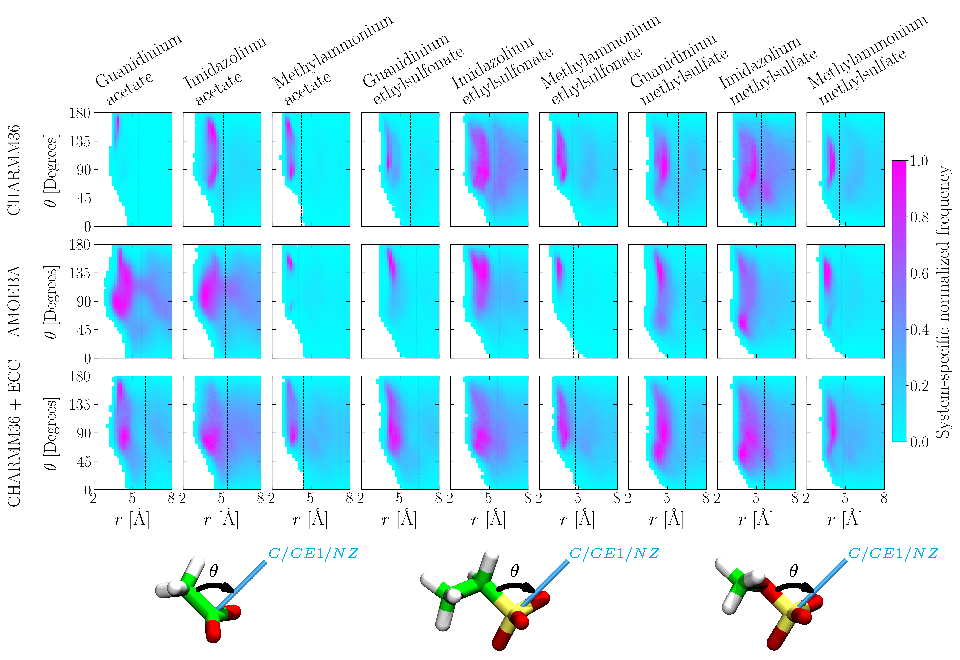
\includegraphics[width=\textwidth]{CEX/final_images/Figure3.pdf}
    \caption{Heat maps of the sampling frequency of configurations defined by the coordinates $(r, \theta)$ for each cation-anion pair (columns) simulated using each force field (rows). Dashed lines represent $R_{Shell}$ and the normalization of sampling frequency is specific to each system. (PMF profiles may be recovered as a projection of these data prior to normalization.)}
    \label{fig:heatmaps_theta_r}
\end{center}
\end{figure*}

When analyzing the same simulation trajectory, the permanent electrostatic contributions are nearly identical for the two FFs, with the largest difference observed in methylsulfate systems, where AMOEBA predicts slightly stronger attraction than CHARMM36 (Fig.~S5). This similarity of permanent electrostatics is intriguing because AMOEBA uses a sophisticated distributed multipole model whereas CHARMM36 uses only point charges at atom centers.\cite{Huang2013, Shi2013} It is also surprising because any implicit inclusion of polarization that may have occurred during the parameterization of CHARMM36 should manifest as a difference between the profiles in Figure~S5. AMOEBA predicts generally weaker van der Waals interactions than CHARMM36 but the magnitude of the difference is relatively small (Fig.~S6). Polarization energies represent the largest quantitative difference between the two FFs in terms of interaction free energy contributions (Fig.~S8). Thus while AMOEBA's more sophisticated multipole treatment of permanent electrostatics does contribute to sampling differences,\cite{Shi2013} polarizability is the primary factor that is responsible for differences in model performance. 

\textbf{Generating-FF analysis:} The PMF may be decomposed as $w = U_{Total} + W_{Solv}$, 
where  $U_{Total} = U_{Elect} + U_{VdW} + U_{Polar}$ is the \emph{in vacuo} interaction energy and $W_{Solv}$ is the solvent-mediated contribution. Unlike the cross-FF analysis, the contributions to $U_{Total}$ were estimated in each simulation trajectory using the trajectory-generating FF and $W_{Solv}$ was found from the PMF by difference; the results are shown in Figures S9-S12. Near the PMF minima, the magnitudes of both $U_{Total}$ and $W_{Solv}$ are on the order of 90 kcal/mol (Figs.~S9 and S10). Thus, it is the fine balance between two large competing contributions that dictates the PMF,\cite{Shi2017} which has a well depth that is typically two orders of magnitude smaller. 

Given the results of the cross-FF analysis, differences between the CHARMM36 and AMOEBA profiles in the generating-FF analysis (Fig.~S9-S12) may be primarily attributed to the sampling differences that polarizability promotes. Permanent electrostatic interactions, which comprise the principal contribution to $U_{Total}$, are similar for CHARMM36 and AMOEBA in most systems (Fig.~S11). However, noticeable discrepancies are apparent in the guanidinium acetate and imidazolium acetate systems, for which CHARMM36 substantially overestimates the magnitude of $U_{Elect}$. The favorable AMOEBA polarization contributions (Fig.~S7) decrease this discrepancy in the $U_{Total}$ profiles for imidazolium acetate (Fig.~S9) but a substantial difference remains for guanidinium acetate. In general, polarization contributions for the other systems and differences in permanent electrostatics lead to more attractive $U_{Total}$ profiles for AMOEBA than CHARMM36 (Fig.~S9). The inferred solvent contribution $W_{Solv}$ necessarily follows the opposite trend (Fig.~S10). 

\textbf{Configurational sampling:}  Differences in configurational sampling were examined more directly for each system by identifying the 3D spaces of the most frequently observed cation positions relative to anions (Fig.~S14) and anion positions relative to cations (Fig.~S15). For example, for guanidinium interacting with acetate or ethylsulfonate (Fig.~S14), the cation samples a small patch of space around the carboxylate group within the CHARMM36 description but this is relaxed in the AMOEBA description.  This trend is approximately reversed for ethylsulfonate. With the ECC correction, no such distinction is evident, suggesting a more promiscuous sampling and hence weaker association.  Similar distinctions can be noted from either the anion's (Fig.~S14) or the cation's perspective (Fig.~S15). To quantify better the sampling differences suggested by the 3D plots, we project the data on an $(r,\theta)$ map (Fig.~\ref{fig:heatmaps_theta_r}, for which $\theta$ is defined in Fig.~\ref{fig:schematic}). For $\theta$ between 90\textdegree \ and 180\textdegree, the carbonyl or sulfonyl oxygen is directed towards the anion.  
   
In general for a given cation, CHARMM36 predicts that configurational preferences become less well-defined as the number of oxygen atoms in the anion increases, i.e., as the charge density decreases. This is as expected on the basis of the dominance of electrostatic interactions.  With some exceptions, the opposite holds for AMOEBA, suggesting a richer interplay of electrostatic interactions arising from charge-charge interactions and polarization effects. The effect of the ECC is inconsistent. 


\textbf{Hydration free energies:} Emergent behavior in ion-pair association is a consequence of the balance between direct interactions and solvent-mediated effects that generally tend to suppress ion-pair formation. The latter arises because there is an energetic penalty for partially dehydrating the interacting ions and reorganizing the nearby solvent structure. Hydration free energies ($\mu^{\rm{ex}}$) may therefore provide a useful complement to inform the understanding of ion pairing phenomena. To this end we estimated $\mu^{\rm{ex}}$ for individual ions using the molecular quasichemical organization of the potential distribution theorem,\cite{Beck2006, Asthagiri2021b, Weber2011, Weber2012} which allows $\mu^{\rm{ex}}$ to be partitioned into physically meaningful contributions as
\begin{eqnarray}
\beta \mu^{\rm{ex}} = \underbrace{- \ln p_0[\phi]}_\text{Packing} + \underbrace{\beta\mu^{\rm{ex}}_{\rm{LR}}[P(\varepsilon \; | \; \phi)]}_\text{Long-range} + \underbrace{\ln x_0[\phi]}_\text{Chemistry}
\label{eq:mqct}
\end{eqnarray}
where the first term represents the free energy required to open a cavity in the solvent to accommodate the ionic solute. Contributions from long-range and short-range solute-solvent interactions are given by the second and third terms, respectively. Each term is a functional of a repulsive potential $\phi$ that is used to condition the solvent up to a maximum range of $\lambda_G$ around the solute, but the sum of the three terms is independent of $\phi$. We use $\lambda_G = 5$~{\AA}, for which the cavity corresponds roughly to the first hydration shell around the solute. Other methodological details for the computation of these terms are provided in Section 4 of the Supporting Information. 

As described elsewhere,\cite{Asthagiri2021b} the estimation of $\mu^{\rm{ex}}$ from molecular quasichemical theory (QCT) offers useful advantages over alchemical approaches because it can better regularize the application of the potential distribution theorem, and it has the substantial added benefit of making hydration free energy contributions physically interpretable. QCT calculations were performed in CHARMM36 and AMOEBA but not in CHARMM36~+~ECC, due to ambiguities in how $\mu^{\rm{ex}}_{\rm{LR}}$ should be corrected for scaled charges. 
 
\begin{figure*}[ht]
    \begin{center}
        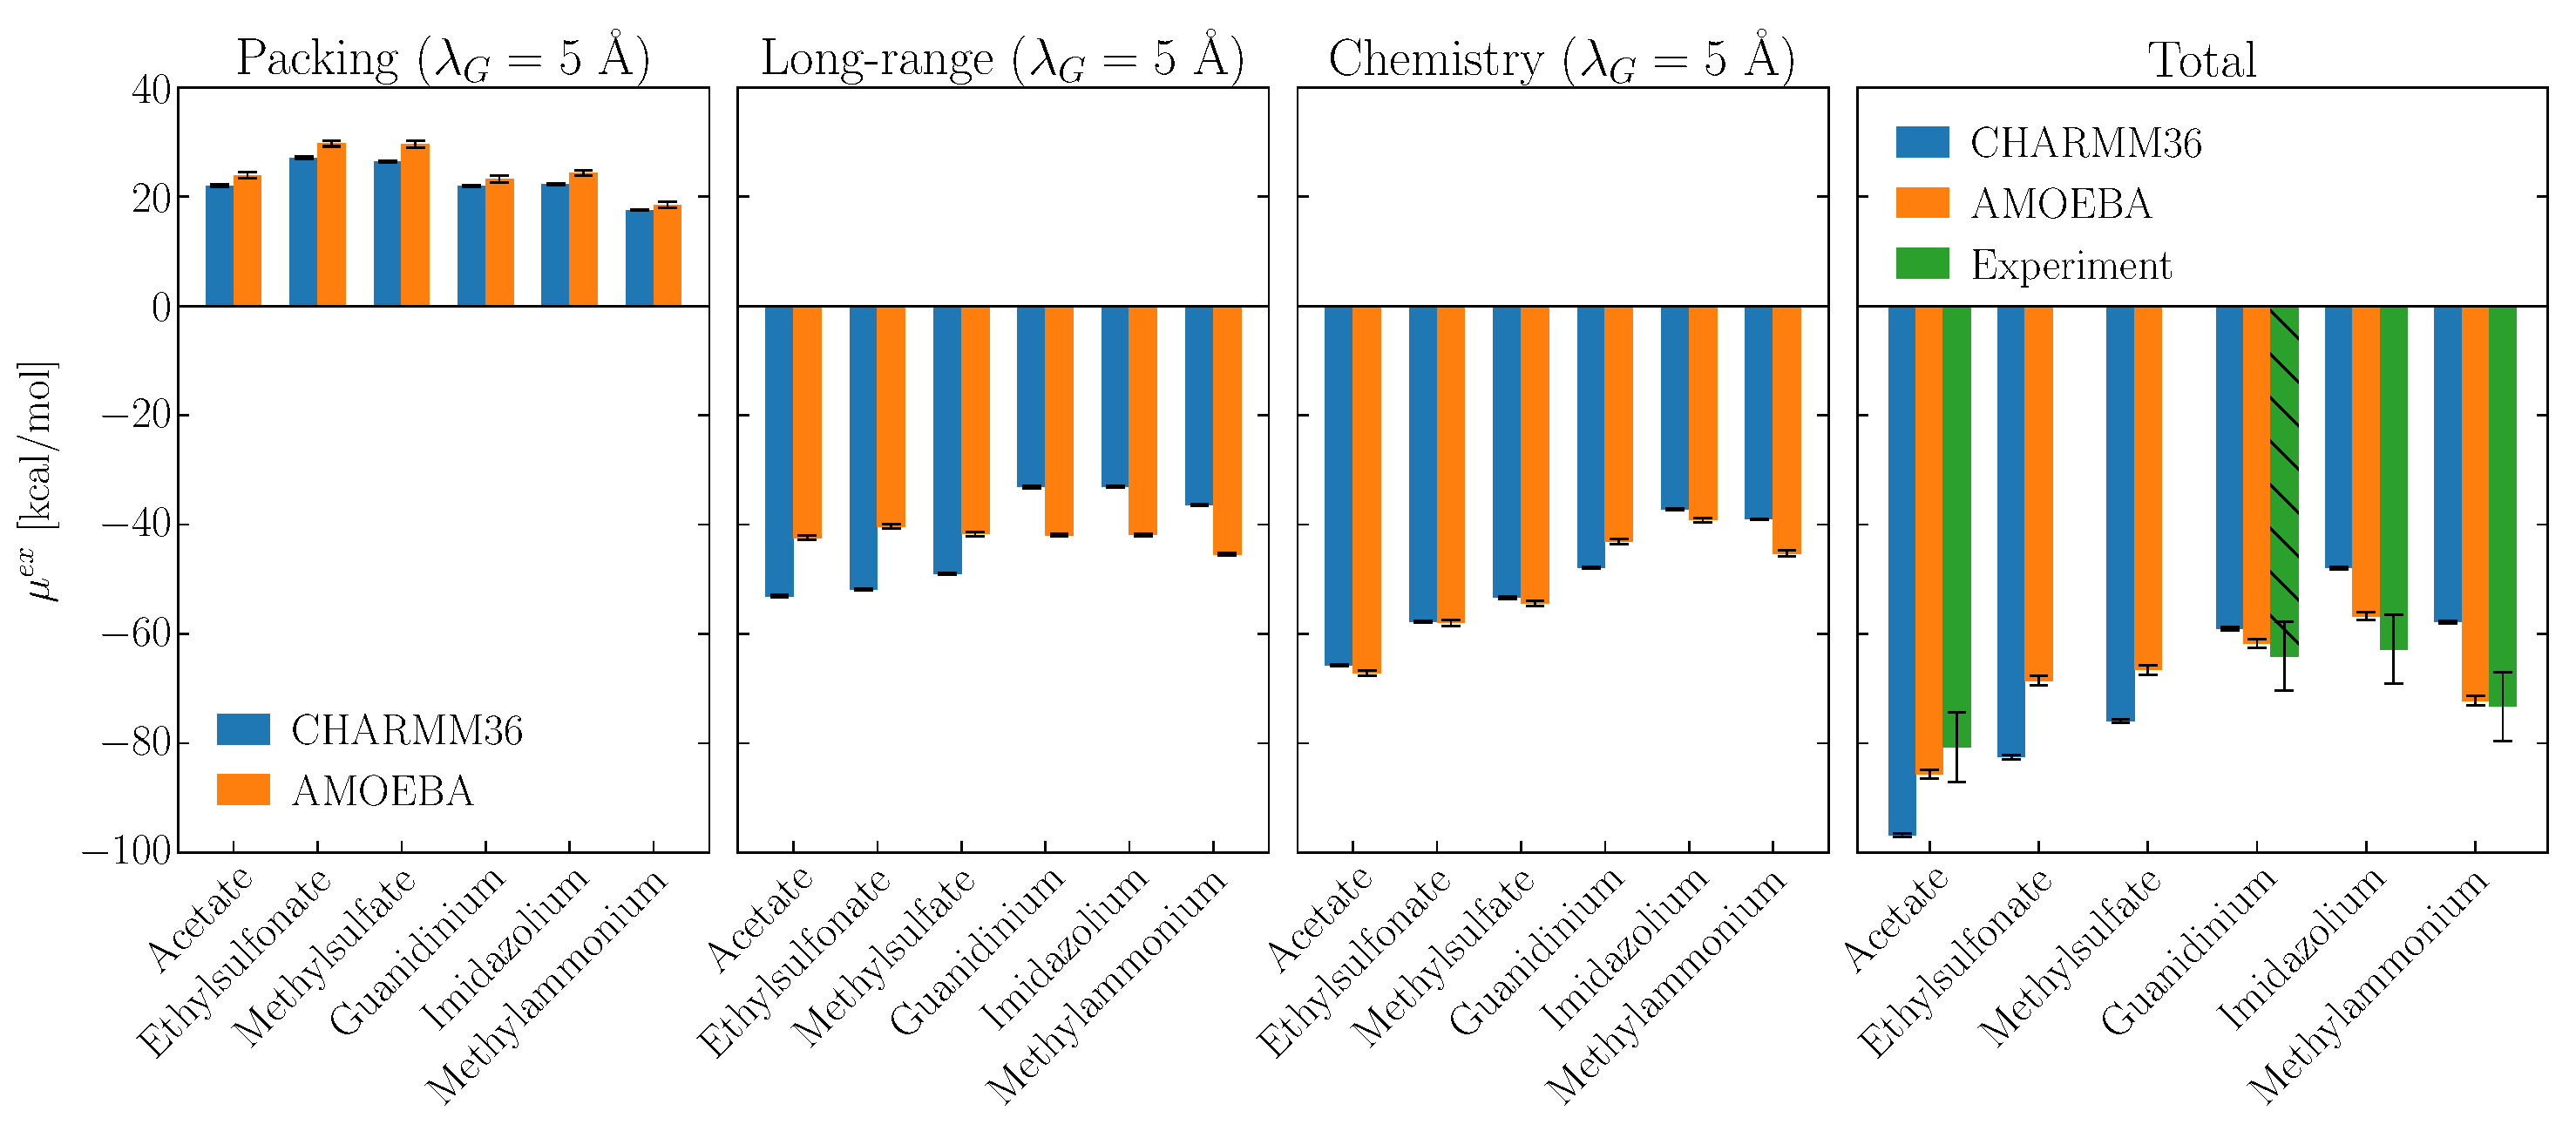
\includegraphics[width=\textwidth]{final_images/Figure4.eps}
        \caption{Partitioning of ion hydration free energies according to molecular quasichemical theory. $\lambda_G = 5$~{\AA} approximately defines the first hydration shell around the solute. Error bars on simulation results represent $2\times$ the standard error of the mean. Where available, experimental data were used to estimate $\mu^{\rm{ex}}$ using a thermodynamic cycle based on a proton hydration free energy of $-260.9 \pm 5.8$ kcal/mol, which represents the mean and standard deviation of 72 independent estimates.\cite{Fossat2021}. Data are given in Tables S3 and S4. Hatched lines indicate that the experimental estimate for guanidinium uses an approximation for the hydration free energy of guanidine (cf.~Table S4).} 
        \label{fig:mqct}
    \end{center}
\end{figure*}
 

Experimental estimates of $\mu^{\rm{ex}}$ may be obtained using a thermodynamic cycle based on proton dissociation, which requires reference to the free energy of hydrating a proton ($\mu^{\rm{ex}}_{H^+}$).\cite{Fossat2021, Lim1991, Pearson1986} However, the value of $\mu^{\rm{ex}}_{H^+}$ is the subject of much uncertainty because extrathermodynamic assumptions must be employed to deconvolute experimentally accessible quantities into anion and cation contributions.\cite{Grossfield2003, Zhang2017, Fossat2021} We have taken $\mu^{\rm{ex}}_{H^+}$ and its uncertainty from a recent report that summarizes 72 independent estimates of the value.\cite{Fossat2021} Literature data exist to make experimental comparisons for the computed $\mu^{\rm{ex}}$ of acetate and the cations,\cite{Cramer1991, Taft1987, Cumming1977, Fujio1981, Settimo2014, Zhang2017, Wolfenden1981, Reif2012, Hunter1998, Rizzo2006, In2005} which are shown alongside simulation results in the rightmost panel of Figure~\ref{fig:mqct} and are detailed in Table~S4. These are comparable to other literature reports that are listed in Table~S5.\cite{Pearson1986, Cramer1991, Gilson1988, Marcus2013, Gokcen2014} Within the appreciable uncertainty, the AMOEBA results agree with experiment. Data for acetate and the cations are also similar to simulation results based on thermodynamic integration.\cite{Lin2018, Fossat2021, Zhang2017}   

We next consider the individual $\mu^{\rm{ex}}$ contributions (Eq.~\ref{eq:mqct}). Uniformly, the packing contribution (i.e., the primitive hydrophobic contribution), to hydration is somewhat stronger (more positive) in AMOEBA than in CHARMM36. With the exception of guanidinium, the chemistry contribution is also stronger (more negative) in AMOEBA than in CHARMM36, which reflects greater ion-water attraction locally. Thus while packing will tend to favor ion-pair complexation in AMOEBA (over CHARMM36), the local attractive contributions will tend to suppress ion-pair formation in AMOEBA (over CHARMM36). 
  
The long-range contribution to hydration proves surprising. This is more favorable for anions than cations in CHARMM36, which is expected based on the positive potential that exists in the center of a cavity due to the preferential orientation of water protons towards the cavity center \cite{Hummer1996,Ashbaugh2000}. However, the trend of long-range interactions found in AMOEBA is nearly reversed. It is well-known that the sign and magnitude of the electric potential that the solvent imposes on the solute charges is sensitive to both the structure of the solvent at the interface and the description of the charge over the solvent molecules \cite{wilsonpratt:1988,doylebeck:2019}; for example, the dipole moment of solvent next to a large anion is itself reduced \cite{Guardia2009}. To probe this, in exploratory calculations for a spherical ion in water, we retrospectively included polarizability and multipole electrostatics in analyzing configurations sampled with a non-polarizable model. The shift is similar to the trend seen in Figure~\ref{fig:mqct} (Long-range). A more thorough investigation is necessarily left for future studies.  
 

\textbf{Matching water affinities:}  To see if we can use the hydration free energies of individual ions to infer ion association, we test the applicability of the empirical law of matching water affinities\cite{Collins1997, Collins2019}. This rule suggests that ions with hydration free energies that are closely matched will tend to associate more readily. Figure~\ref{fig:volcano} shows that when using hydration free energies obtained from AMOEBA (which are closer to experimental estimates), there is a clear correlation between the difference in hydration free energy and the PMF well depth. The greater the difference in hydration free energy, the lower is the ion pair association affinity, which is reminiscent of experimentally observed trends in salt dissolution free energies.\cite{Collins1997} With CHARMM36 there is considerable scatter and the law of matching water affinities does not seem to hold. Although CHARMM36 predicts correctly that acetate is the most energetically expensive anion to dehydrate, it predicts incorrectly that cation interactions will be strongest with acetate. Overall, the results suggest that the empirical law of matching water affinities could be used in inferring ion-pairing, and hence potential protein adsorption on CEX matrices, provided the hydration of the individual ions is itself well captured (Fig.~\ref{fig:mqct}).

\begin{figure*}[ht]
    \begin{center}
        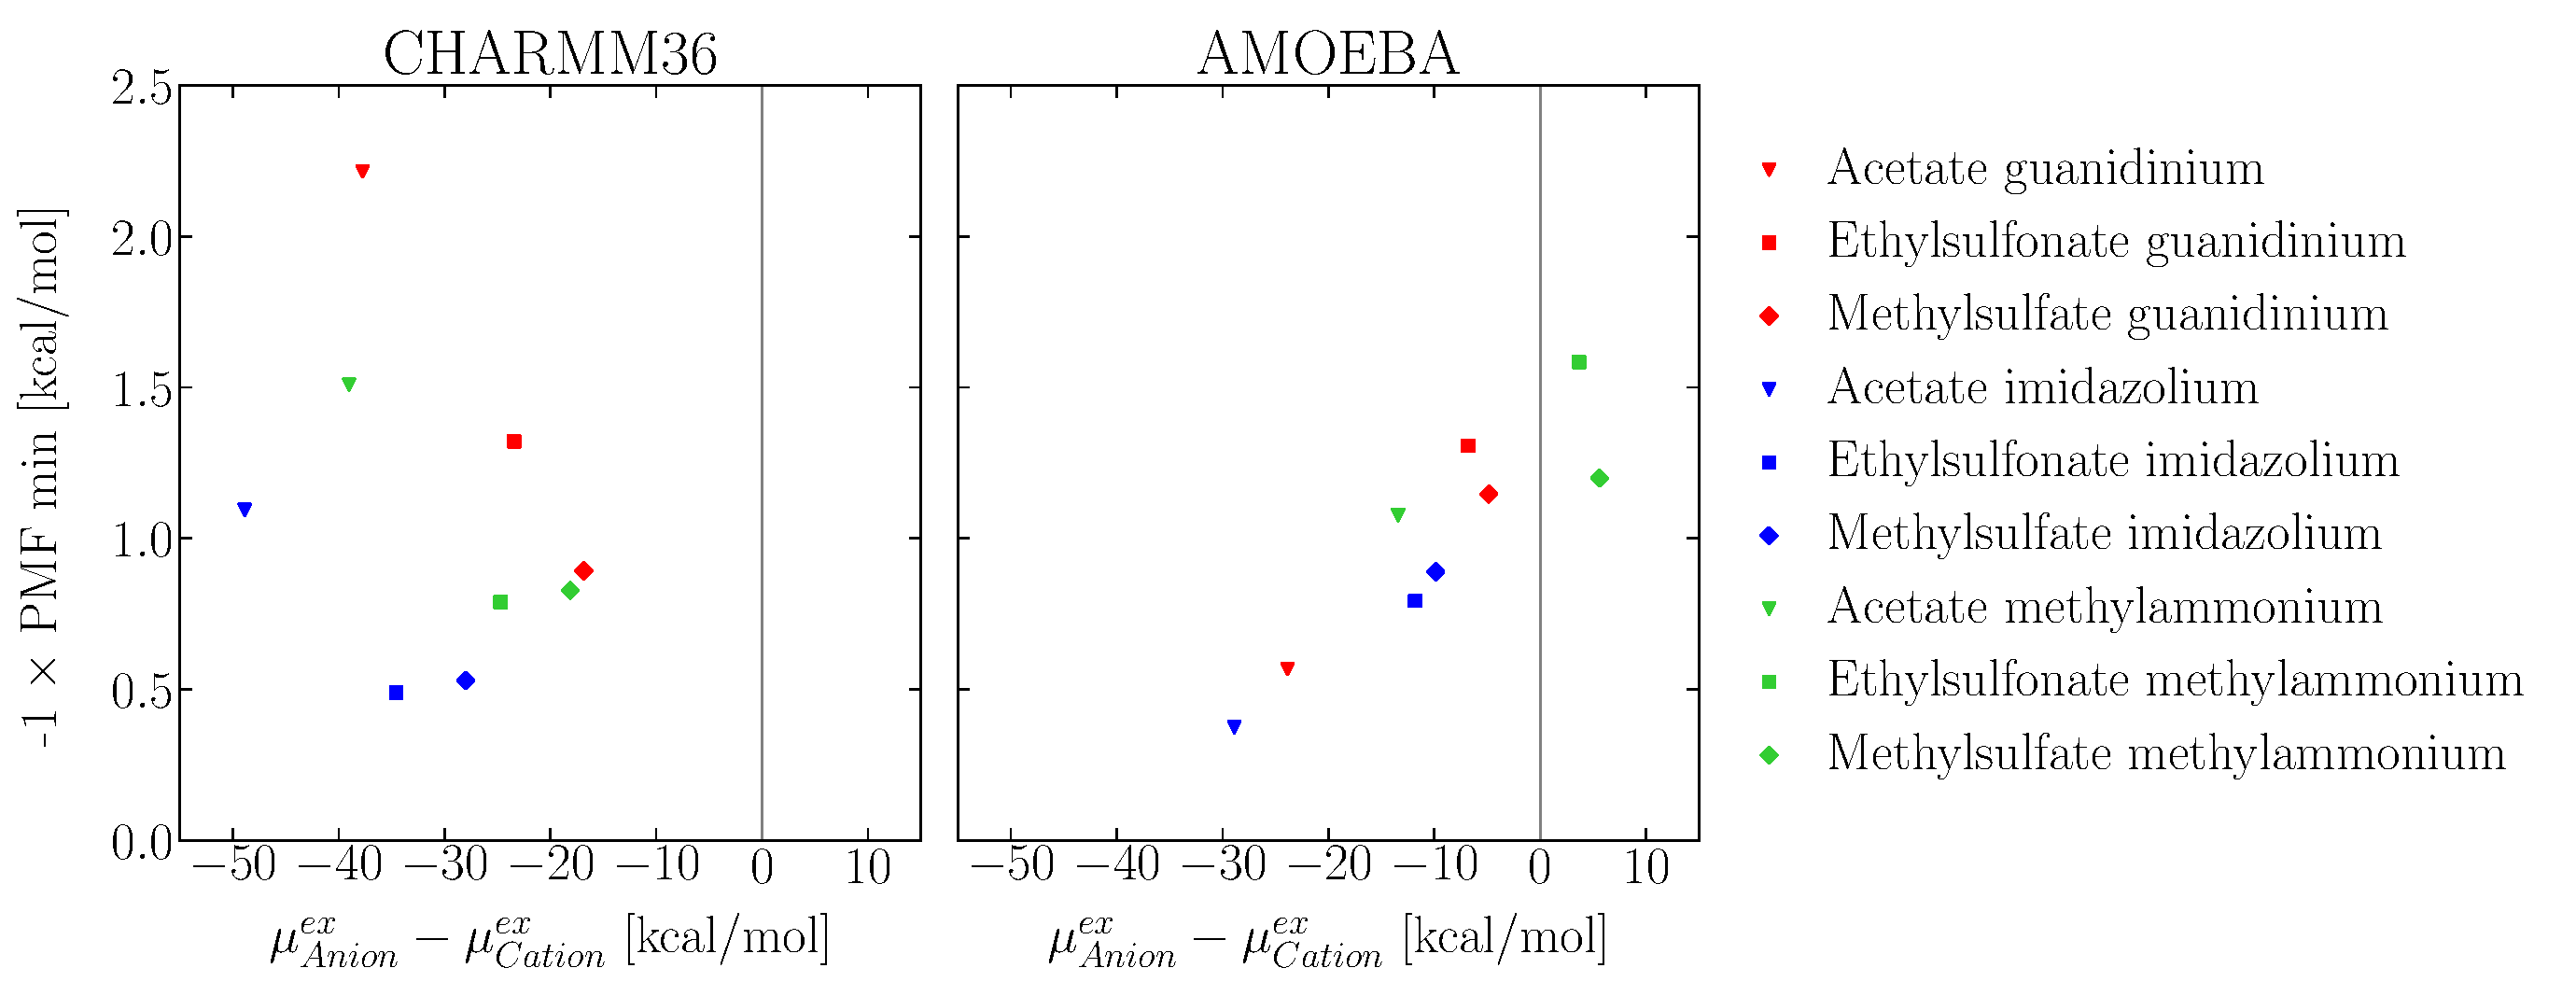
\includegraphics[width=\textwidth]{final_images/Figure5.eps}
        \caption{Comparison of potential of mean force well depths ($-1 \times \text{PMF min}$) with the difference in hydration free energies between the corresponding anion and cation as computed using CHARMM36 and AMOEBA. Marker sizes are close to $2\times$ the standard error of the mean (error not shown for marker readability).}
        \label{fig:volcano}
    \end{center}
\end{figure*}

In conclusion, the present study suggests that the physics of polarizability is critical in determining why positively charged amino acid side chains bind more strongly to sulfate and sulfonate moieties than carboxylate groups, despite the fact that carboxylate has a more negative surface charge density and ought to interact more strongly with cations. The carboxylate moiety is more energetically expensive to dehydrate but predicting this is only half of the puzzle. Subtle polarization effects are required to capture experimental trends because it is the fine difference between two large competing potentials (i.e., electrostatic attraction and solvent opposition) that underlies ion complexation in solution. Although the ECC can sometimes improve this balance in classical FFs, it may also promote spuriously promiscuous configurational sampling. Polarizability leads to qualitatively distinct configurational preferences that are expected to be broadly relevant to protein electrostatic interactions.



\section{Supporting Information} 
    Supporting information includes methods and supplementary results for (1) unbiased simulations, (2) \emph{in vacuo} energy analyses (including cross-FF and generating-FF analyses), (3) configurational sampling analyses (including 3D maps, coordinate definitions and supplementary heat maps), (4) molecular QCT simulations and (5) experimental estimates of $\mu^{\rm{ex}}$ based on a thermodynamic cycle (PDF); simulation parameter files that were generated to supplement routinely accessible inputs are available online at \url{https://github.com/ceherman/CEX_polarizability/}

    % The parameters files are also in the .zip archive in this project
    
\section{Acknowledgements}
    We thank Tom Beck (ORNL) for helpful discussions. 
    This research was supported in part through the use of DARWIN computing system: DARWIN – A Resource for Computational and Data-intensive Research at the University of Delaware and in the Delaware Region, which is supported by NSF under Grant Number: 1919839, Rudolf Eigenmann, Benjamin E. Bagozzi, Arthi Jayaraman, William Totten, and Cathy H. Wu, University of Delaware, 2021, URL: https://udspace.udel.edu/handle/19716/29071

    This research used resources of the Oak Ridge Leadership Computing Facility at the Oak Ridge National Laboratory, which is supported by the Office of Science of the U.S. Department of Energy under Contract No. DE-AC05-00OR22725.
    

\bibliography{myref}
	
\end{document} 
